
\documentclass[12pt]{article}
\usepackage{tikz}
\usetikzlibrary{shapes}
\usetikzlibrary{arrows}

\begin{document}

\thispagestyle{empty}
\setlength{\fboxrule}{0.01pt}
\setlength{\fboxsep}{4pt}

\fcolorbox{white}{white}{

\newcommand{\sys}[1]{\emph{#1}}

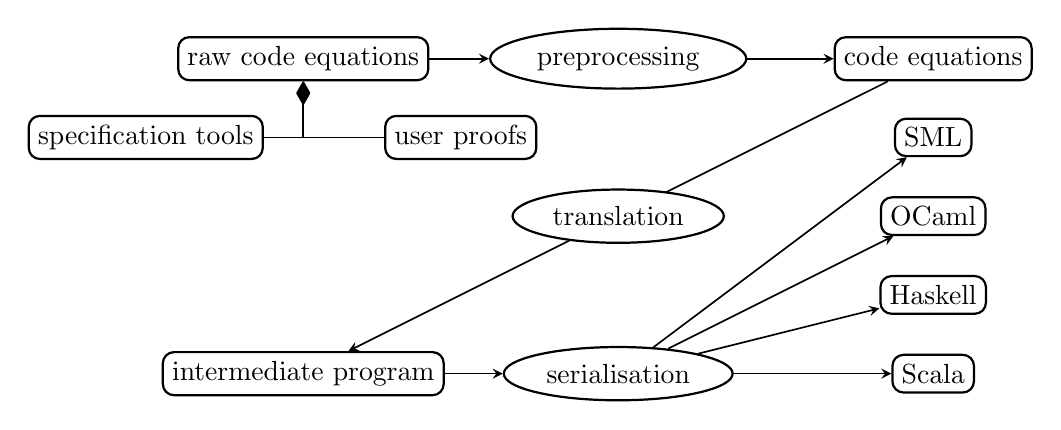
\begin{tikzpicture}[x = 4cm, y = 1cm]
  \tikzstyle positive=[color = black, fill = white];
  \tikzstyle negative=[color = white, fill = black];
  \tikzstyle entity=[rounded corners, draw, thick];
  \tikzstyle process=[ellipse, draw, thick];
  \tikzstyle arrow=[-stealth, semithick];
  \node (spec) at (0, 3) [entity, positive] {specification tools};
  \node (user) at (1, 3) [entity, positive] {user proofs};
  \node (spec_user_join) at (0.5, 3) [shape=coordinate] {};
  \node (raw) at (0.5, 4) [entity, positive] {raw code equations};
  \node (pre) at (1.5, 4) [process, positive] {preprocessing};
  \node (eqn) at (2.5, 4) [entity, positive] {code equations};
  \node (iml) at (0.5, 0) [entity, positive] {intermediate program};
  \node (seri) at (1.5, 0) [process, positive] {serialisation};
  \node (SML) at (2.5, 3) [entity, positive] {\sys{SML}};
  \node (OCaml) at (2.5, 2) [entity, positive] {\sys{OCaml}};
  \node (Haskell) at (2.5, 1) [entity, positive] {\sys{Haskell}};
  \node (Scala) at (2.5, 0) [entity, positive] {\sys{Scala}};
  \draw [semithick] (spec) -- (spec_user_join);
  \draw [semithick] (user) -- (spec_user_join);
  \draw [-diamond, semithick] (spec_user_join) -- (raw);
  \draw [arrow] (raw) -- (pre);
  \draw [arrow] (pre) -- (eqn);
  \draw [arrow] (eqn) -- node (transl) [process, positive] {translation} (iml);
  \draw [arrow] (iml) -- (seri);
  \draw [arrow] (seri) -- (SML);
  \draw [arrow] (seri) -- (OCaml);
  \draw [arrow] (seri) -- (Haskell);
  \draw [arrow] (seri) -- (Scala);
\end{tikzpicture}

}

\end{document}
